\documentclass{article}
\usepackage{spconf,amsmath,graphicx}
\usepackage[utf8]{inputenc}
\usepackage{xcolor}
\usepackage{blindtext}
\usepackage{enumitem}
\usepackage{booktabs}
\usepackage{hyperref}
\usepackage[caption=false]{subfig}
\usepackage{caption} 
\captionsetup[table]{skip=8pt}
%\usepackage{makecell}
%\renewcommand\theadalign{bc}
%\renewcommand\theadfont{\bfseries}
%\renewcommand\theadgape{\Gape[4pt]}
%\renewcommand\cellgape{\Gape[4pt]}
% For subfig.sty:
 \let\MYorigsubfloat\subfloat
 \renewcommand{\subfloat}[2][\relax]{\MYorigsubfloat[]{#2}}
% Example definitions.
% --------------------
\def\x{{\mathbf x}}
\def\L{{\cal L}}
\usepackage{dblfloatfix}

\newcommand{\ines}{\textcolor{black}}

% Title.
% ------
\title{COST-SENSITIVE LOSS MINIMIZATION FOR RETINAL IMAGE ANALYSIS}


\name{Adrian Galdran$^{\star, \dagger}$, J. Dolz$^{\dagger}$, A. Christodoulidis$^{\ddagger}$, H. Chakor$^{\ddagger}$, H. Lombaert$^{\dagger}$, I. ben Ayed$^{\dagger}$
\thanks{Corresponding author: Adrian Galdran (agaldran@bournemouth.ac.uk).
}
}
\address{$^{\star}$ 
Bournemouth University, UK \\
$^{\dagger}$ École de Technologie Supérieure, University of Quebec, Canada
\\
${\ddagger}$ Diagnos INC., Quebec, Canada
}


\begin{document}
%\ninept
%
\maketitle
%
\begin{abstract}
This short paper includes a description of the method employed by our team to address the DEEP-DR challenge. 
We participate in each of the three sub-challenges.
While our solution for sub-challenge 1 (DR grading from fundus images) and sub-challenge 3 (DR grading from UW images) is based on similar ideas, we introduce a different strategy for sub-challenge 2 (fundus image quality assessment). 
In the first case, we rely on a methodology based on Cost-Sensitive regularization adapted to standard CNNs for better performing DR grading. 
This consists of attaching an extra term that acts as a regularizer to standard classification losses, with the goal of imposing greater penalties on predicted grades when they are farther away from the true grade associated to a particular image.
For the latter, we train five different CNNs, four of them meant to solve each of the sub-tasks in sub-challenge 2 independently, and a fifth one that solves the four sub-tasks simultaneously, sharing the same convolutional weights and internal representation but with four different predictive streams in the last part of the architecture.
Our approach performs reasonably well in our internal validation tests as well as in the online validation set. 
Code to reproduce our results is released at \url{github.com/agaldran/deepdr}.
\end{abstract}
%
\begin{keywords}
Diabetic Retinopathy Grading, Cost-Sensitive Classification, Retinal Image Quality Assessment, Ultra-Wide Field Retinal Imaging
\end{keywords}

\begin{figure*}[t]
\centering
\subfloat[]{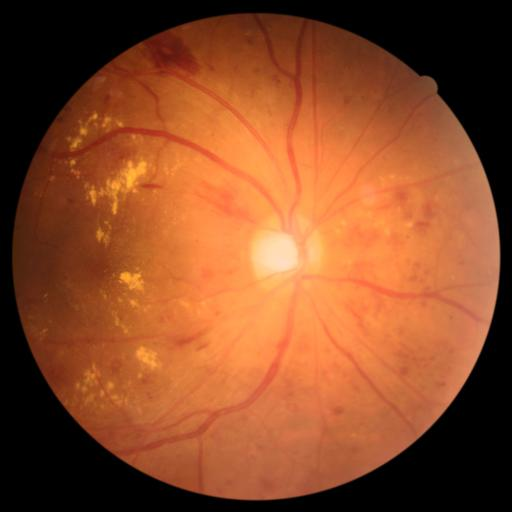
\includegraphics[width = 0.24\textwidth]{images/12_r1.jpg}
\label{fig_deg_1}}
\hfil
\subfloat[]{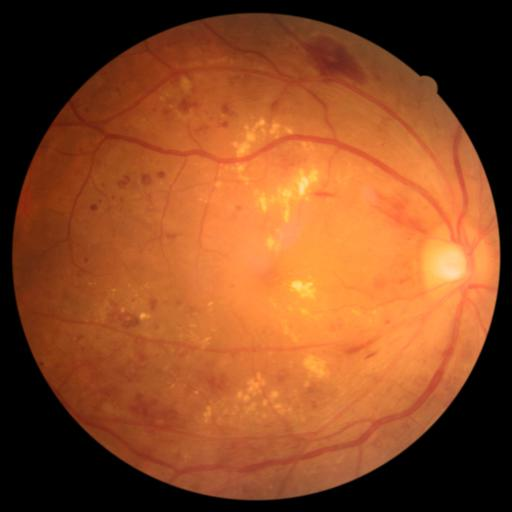
\includegraphics[width = 0.24\textwidth]{images/12_r2.jpg}
\label{fig_deg_2}}
\hfil
\subfloat[]{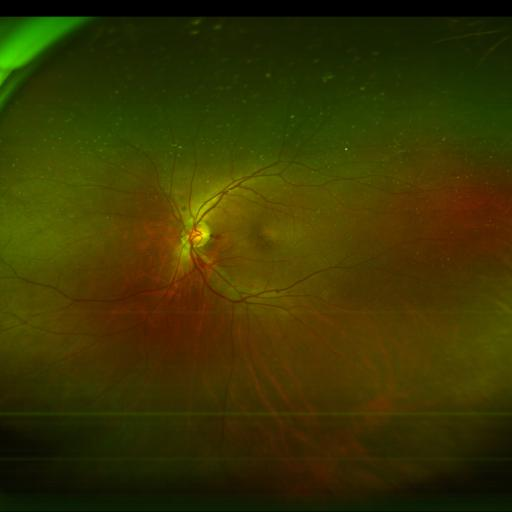
\includegraphics[width = 0.24\textwidth]{images/18_l2.jpg}
\label{fig_deg_3}}
\hfil
\subfloat[]{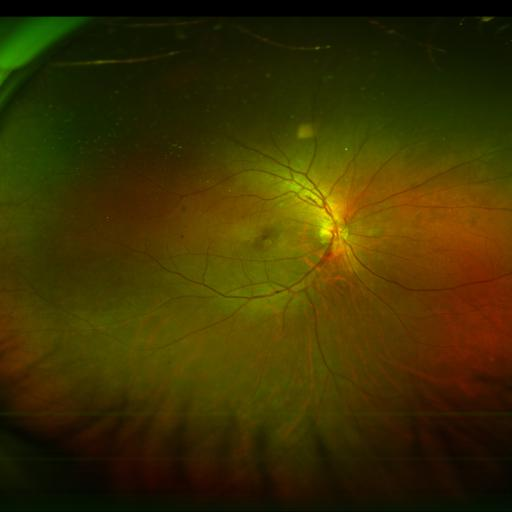
\includegraphics[width = 0.24\textwidth]{images/18_r1.jpg}
\label{fig_deg_4}}
\caption{Different image modalities involved in this challenge: (a) Optic Disc-centered retinal fundus image, (b) Macula-centered retinal fundus image, (c) Optic Disc-centered UW-Field retinal image, and (d) Macula-centered Ultra-Wild Field retinal image.}
\label{fig_samples}
\end{figure*}

\section{Introduction}
Diabetes is regarded as a global eye health issue, with a steadily increasing world-wide affected population, estimated to reach 630 million individuals by 2045 \cite{noauthor_who_nodate}. Diabetic Retinopathy (DR) is a complication of standard diabetes, caused by damage to vasculature within the retina. DR shows early signs in the form of swelling micro-lesions that destroy small vessels and release blood into the retina. More advanced DR stages are characterized by the appearance of other more noticeable symptoms, e.g. proliferation of neo-vessels, which may lead to the detachment of the retinal layer and eventually
permanent sight loss. Retinal images acquired with fundus cameras are the tool of choice for capturing and depicting all these early symptoms, thereby representing an effective diagnostic tool \cite{fenner_advances_2018}. 

This challenge is composed by three sub-challenges, namely DR grading from standard fundus images (Challenge 1), from Ultra-Wield Field retinal images (Challenge 3), and retinal fundus image quality assessment (Challenge 2). 
In addition, for each eye the organization provides a retinal image acquired when the optic disc is located in the center of the picture, and a complementary image where the acquisition is with the macula on the center, as shown in Figure 1. Our team  participates in all three Challenges. 
In the following we detail our proposed solution for each task.

\section{Methodology}
\subsection{DR grading from standard Eye Fundus Images}
For the DR grading, labels are distributed in an heterogeneous manner, as a consequence of the structure underlying the diagnosis of this disease.
As an example, a image annotated as Mild DR has a label closer to the label of a healthy image than to the label of an image showing signs of Proliferative DR.
For this reason, we employ a special technique that accounts for such label structure, which we have introduced in \cite{galdran_cost-sensitive_2020}.
Briefly, we consider a model $U$ producing a prediction $U(x)=\hat{y} \in [0,1]\times \displaystyle \ldots \times[0,1]$, and an associated ground-truth label $y$. 

Our goal is to introduce in the loss computation of a standard CNN trained by backpropgation a cost matrix $M$ that encodes a null cost for a prediction such that $\hat{y}=y_j$, but cost that increases along with the distance $\|y - \hat{y}\|$. 
A simple approach to achieve such increasing label-dependent penalty is by encoding in each row of $M$ those costs, and then computing the scalar product of $\hat{y}$ with the row of $M$ corresponding to $y$, i.e. $\mathcal{L}(y,\hat{y})=\langle M(y,\cdot), \hat{y} \rangle$. 
However, due to the high imbalance of the DR grading problem (with typically few examples of classes DR1, DR3, and DR4) in our experiments we prefer to combine a Cost-Sensitive term with a base loss as follows:
\begin{equation}\label{cs_loss}
\mathcal{L}^{cs}(y,\hat{y}) = \mathcal{L}^{base}(\hat{y},y) + \lambda \langle M^{(2)}(y,\cdot), \hat{y} \rangle, \ \ \  M_{ij}=\|i-j\|_2.
\end{equation}
In the above equation, we have selected the $L^1$-based ground cost matrix $M$, since in our internal validation experiments we noticed this configuration was the one attaining greater quadratic-weighted kappa score, which is the main performance metric in this competition.

In this work, we consider a standard CNN archtitecture, namely ResNet-50 \cite{he_deep_2016}, as it
has established in recent years as a standard in computer vision applications. 
We train this model by using the above regularization and several loss functions as a base error measure, namely Cross-Entropy, Focal Loss \cite{lin_focal_2020}, and Non-Uniform Label Smoothing \cite{galdran_non-uniform_2020}. 
Our models are trained starting from weights pre-trained for the Kaggle Eyepacs competition dataset, based on the above loss function and architecture for each of the two image subsets (OD-centered and macula-centered) independently. 
In addition, we also train a third model on the entire dataset (OD+Macula). 
In test time, for a particular image centered, e.g., in the OD, we combine predictions coming from models trained on OD-centered images with predictions coming from training on both kind of images.

\subsection{Fine-Tuning for UW-image recognition}
The Ultra-Wide Field retinal image dataset on this sub-challenge contains significantly less training examples than the standard fundus image dataset.
For this reason, we fine-tune our best models from the previous section on this new task, again using Cost-Senstive regularization.
In addition, we keep the same strategy as outlined above: we train separate models for OD-centered images, macula-centered  images, and a combination of both.

\subsection{Image Quality Assessment from Retinal Fundus Images}
This sub-challenge encompasses four different sub-tasks, each of them accounting for a different kind of image degradation,and the task is to categorize each degradation into a variable number of classes, ranging from two (Overall Quality) to six (Field Definition). 

In order to potentially improve generalization ability, we train five different models on the available training data. 
First, we train four different image quality assessment models meant to solve each of the four different sub-tasks independently. 
Then we train a last model that solves jointly the four problems. This is done by implementing four different prediction branches towards the end of our architecture, as illustrated in Fig. \ref{fig_architecture}.
In test time, for each sub-task we combine predictions generated from the model trained specifically for that particular task with the model trained in a multi-task manner.
We hypothesize that this approach contributes to the learning of useful representations that can take advantage of certain correlation existing between the different sub-tasks that compose this part of the competition.

\begin{figure*}[h]
\centering
\includegraphics[width=0.9\textwidth]{images/fig1_new.pdf}
\caption{Our multi-task architecture, generating simultaneously predictions for all four sub-tasks in sub-challenge 2.}
\label{fig_architecture}
\end{figure*}

%
%\begin{table*}[!b]  %* for the two columns
	%% increase table row spacing, adjust to taste
	%\renewcommand{\arraystretch}{1.3}	
	\centering
	%\sisetup{detect-weight=true,detect-inline-weight=math}
%\setlength\tabcolsep{5pt}	
\caption{Performance comparison between the technique from \cite{moccia_learning-based_2018} and fine-tuned SqueezeNet. \textbf{IQR}: Inter-Quartile Range.}
\begin{tabular}{l cccccc c cccccc }
%\toprule
 & \multicolumn{6}{c}{\textbf{Feature-Based + SVM} \cite{moccia_learning-based_2018} } & & \multicolumn{6}{c}{\textbf{Proposed (SqueezeNet-based)}} \\
\cmidrule(lr){2-7} \cmidrule(lr){9-14}
& \textbf{I}   & \textbf{B}  & \textbf{S} & \textbf{U} & \textbf{Median} &\textbf{IQR}& &\textbf{I}   & \textbf{B}  & \textbf{S} & \textbf{U} & \textbf{Median} &\textbf{IQR}\\
%\midrule
\cmidrule(lr){1-7} \cmidrule(lr){9-14}
\textbf{Precision}  & 0.91 & 0.76 & 0.78 & 0.76 & 0.77 & 0.09 & & 0.97 & 0.94 & 0.93 & 0.97 & 0.95 & 0.03 \\
\textbf{Recall}       & 0.91 & 0.83 & 0.62 & 0.85 & 0.84 & 0.16 & & 1 & 0.94 & 0.91 & 0.94 & 0.94 & 0.02 \\
\textbf{F1-Score}   & 0.91 & 0.79 & 0.69 & 0.80 & 0.80 & 0.12 & & 0.98 & 0.94 & 0.91 & 0.95 & 0.95 & 0.03 \\
\bottomrule
\end{tabular}
\label{tab_1_results}
\end{table*}%* for the two columns

%
\section{Experimental Evaluation}
Our models are tested on $20\%$ of the test data, which has been made available online. 
Final results will be added to the manuscript when our approach is tested against data released for the on-site challenge.
%
\section{Discussion and Future Work}
From Fig. \ref{fig_rocs}, we observe that the three fine-tuned CNNs tested in this work exceed previously reported performance in the NBI-InfFrames dataset by a wide margin. Performance metrics demonstrate that the weights learned for the task of natural image classification are indeed useful for identifying informative laryngoscopic frames. Interestingly, the simplest of the three employed models delivered the highest performance, revealing that too much complexity may lead to a slight overfitting, and it may be preferable to opt for moderately expressive architectures to increase generalizability in this setting.

The analysis reported in Table \ref{tab_1_results} shows that both the approach introduced in \cite{moccia_learning-based_2018} and SqueezeNet suffer when assigning the correct category to uninformative frames, whereas the classification into informative frames was almost perfect for the case of the CNN. When classifying uninformative frames into blurry, containing specularities/saliva, and underexposed, the fine-tuned SqueezeNet achieved a slightly lower performance, although the overall median accuracy was high enough so as to consider this simple CNN as an excellent baseline for further research on laryngoscopic frame classification, with a $94\%$ median recall and a $95\%$ median precision. In addition, the inter-quartile range was also lower than in \cite{moccia_learning-based_2018} for every measure, pointing to a great robustness of the proposed approach in this problem.

Our findings indicate that a simple CNN like SqueezeNet suffices to successfully solve the task of informative frame classification in laringoscopies. In addition, the moderate complexity of SqueezeNet turns this approach into an ideal candidate for its introduction in clinical workflows. Its lightweight memory requirements (less than 0.5 MB) enable its embedding even in portable devices, and its fast inference time (one order of magnitude lower than previously reported times) allows for the addition of further image processing or computer vision post-processing modules (\textit{e.g.} abnormality detectors or image quality enhancement techniques) without hindering the potential for real-time execution.

The next step will consist of considering full video processing, where the temporal dimension of the data could be also taken into account by means of Recurrent Neural Networks coupled with CNNs. This may further increase the consistency of predictions, and enable an improved analysis of laryngoscopic frame visual content. Image processing techniques for restoring visibility on un-informative frames based on different exposures \cite{galdran_image_2018} will also be considered.

%\section{Conclusions and Future Work}
Wrapping everything up, summarize what we did here, stress benefits and good performance.

Also, work that could be done now.



\bibliographystyle{abbrv}
%\bibliographystyle{IEEEbib}
%\bibliography{strings,refs}
\bibliography{isbi20_deepdr}

\end{document}